%!TeX root=../wowtop.tex

\ArtChapter[The Death of the Curate]{21head}

\lettrine[lines=4,findent=2pt]{I}{t} was on the sixth day of our imprisonment that I peeped for the last time, and presently found myself alone. Instead of keeping close to me and trying to oust me from the slit, the curate had gone back into the scullery. I was struck by a sudden thought. I went back quickly and quietly into the scullery. In the darkness I heard the curate drinking. I snatched in the darkness, and my fingers caught a bottle of burgundy.

For a few minutes there was a tussle. The bottle struck the floor and broke, and I desisted and rose. We stood panting and threatening each other. In the end I planted myself between him and the food, and told him of my determination to begin a discipline. I divided the food in the pantry, into rations to last us ten days. I would not let him eat any more that day. In the afternoon he made a feeble effort to get at the food. I had been dozing, but in an instant I was awake. All day and all night we sat face to face, I weary but resolute, and he weeping and complaining of his immediate hunger. It was, I know, a night and a day, but to me it seemed—it seems now—an interminable length of time.

And so our widened incompatibility ended at last in open conflict. For two vast days we struggled in undertones and wrestling contests. There were times when I beat and kicked him madly, times when I cajoled and persuaded him, and once I tried to bribe him with the last bottle of burgundy, for there was a rain-water pump from which I could get water. But neither force nor kindness availed; he was indeed beyond reason. He would neither desist from his attacks on the food nor from his noisy babbling to himself. The rudimentary precautions to keep our imprisonment endurable he would not observe. Slowly I began to realise the complete overthrow of his intelligence, to perceive that my sole companion in this close and sickly darkness was a man insane.

From certain vague memories I am inclined to think my own mind wandered at times. I had strange and hideous dreams whenever I slept. It sounds paradoxical, but I am inclined to think that the weakness and insanity of the curate warned me, braced me, and kept me a sane man.

On the eighth day he began to talk aloud instead of whispering, and nothing I could do would moderate his speech.

»It is just, O God!« he would say, over and over again. »It is just. On me and mine be the punishment laid. We have sinned, we have fallen short. There was poverty, sorrow; the poor were trodden in the dust, and I held my peace. I preached acceptable folly—my God, what folly!—when I should have stood up, though I died for it, and called upon them to repent—repent!\textellipsis Oppressors of the poor and needy\textellipsis! The wine press of God!«

Then he would suddenly revert to the matter of the food I withheld from him, praying, begging, weeping, at last threatening. He began to raise his voice—I prayed him not to. He perceived a hold on me—he threatened he would shout and bring the Martians upon us. For a time that scared me; but any concession would have shortened our chance of escape beyond estimating. I defied him, although I felt no assurance that he might not do this thing. But that day, at any rate, he did not. He talked with his voice rising slowly, through the greater part of the eighth and ninth days—threats, entreaties, mingled with a torrent of half-sane and always frothy repentance for his vacant sham of God's service, such as made me pity him. Then he slept awhile, and began again with renewed strength, so loudly that I must needs make him desist.

»Be still!« I implored.

He rose to his knees, for he had been sitting in the darkness near the copper.

»I have been still too long,« he said, in a tone that must have reached the pit, »and now I must bear my witness. Woe unto this unfaithful city! Woe! Woe! Woe! Woe! Woe! To the inhabitants of the earth by reason of the other voices of the trumpet\longdash«

»Shut up!« I said, rising to my feet, and in a terror lest the Martians should hear us. »For God's sake\longdash«

»Nay,« shouted the curate, at the top of his voice, standing likewise and extending his arms. »Speak! The word of the Lord is upon me!«

In three strides he was at the door leading into the kitchen.

»I must bear my witness! I go! It has already been too long delayed.«

I put out my hand and felt the meat chopper hanging to the wall. In a flash I was after him. I was fierce with fear. Before he was halfway across the kitchen I had overtaken him. With one last touch of humanity I turned the blade back and struck him with the butt. He went headlong forward and lay stretched on the ground. I stumbled over him and stood panting. He lay still.

Suddenly I heard a noise without, the run and smash of slipping plaster, and the triangular aperture in the wall was darkened. I looked up and saw the lower surface of a handling-machine coming slowly across the hole. One of its gripping limbs curled amid the debris; another limb appeared, feeling its way over the fallen beams. I stood petrified, staring. Then I saw through a sort of glass plate near the edge of the body the face, as we may call it, and the large dark eyes of a Martian, peering, and then a long metallic snake of tentacle came feeling slowly through the hole.

I turned by an effort, stumbled over the curate, and stopped at the scullery door. The tentacle was now some way, two yards or more, in the room, and twisting and turning, with queer sudden movements, this way and that. For a while I stood fascinated by that slow, fitful advance. Then, with a faint, hoarse cry, I forced myself across the scullery. I trembled violently; I could scarcely stand upright. I opened the door of the coal cellar, and stood there in the darkness staring at the faintly lit doorway into the kitchen, and listening. Had the Martian seen me? What was it doing now?

Something was moving to and fro there, very quietly; every now and then it tapped against the wall, or started on its movements with a faint metallic ringing, like the movements of keys on a split-ring. Then a heavy body—I knew too well what—was dragged across the floor of the kitchen towards the opening. Irresistibly attracted, I crept to the door and peeped into the kitchen. In the triangle of bright outer sunlight I saw the Martian, in its Briareus of a handling-machine, scrutinizing the curate's head. I thought at once that it would infer my presence from the mark of the blow I had given him.

\begin{figure}[tbp]
\centering
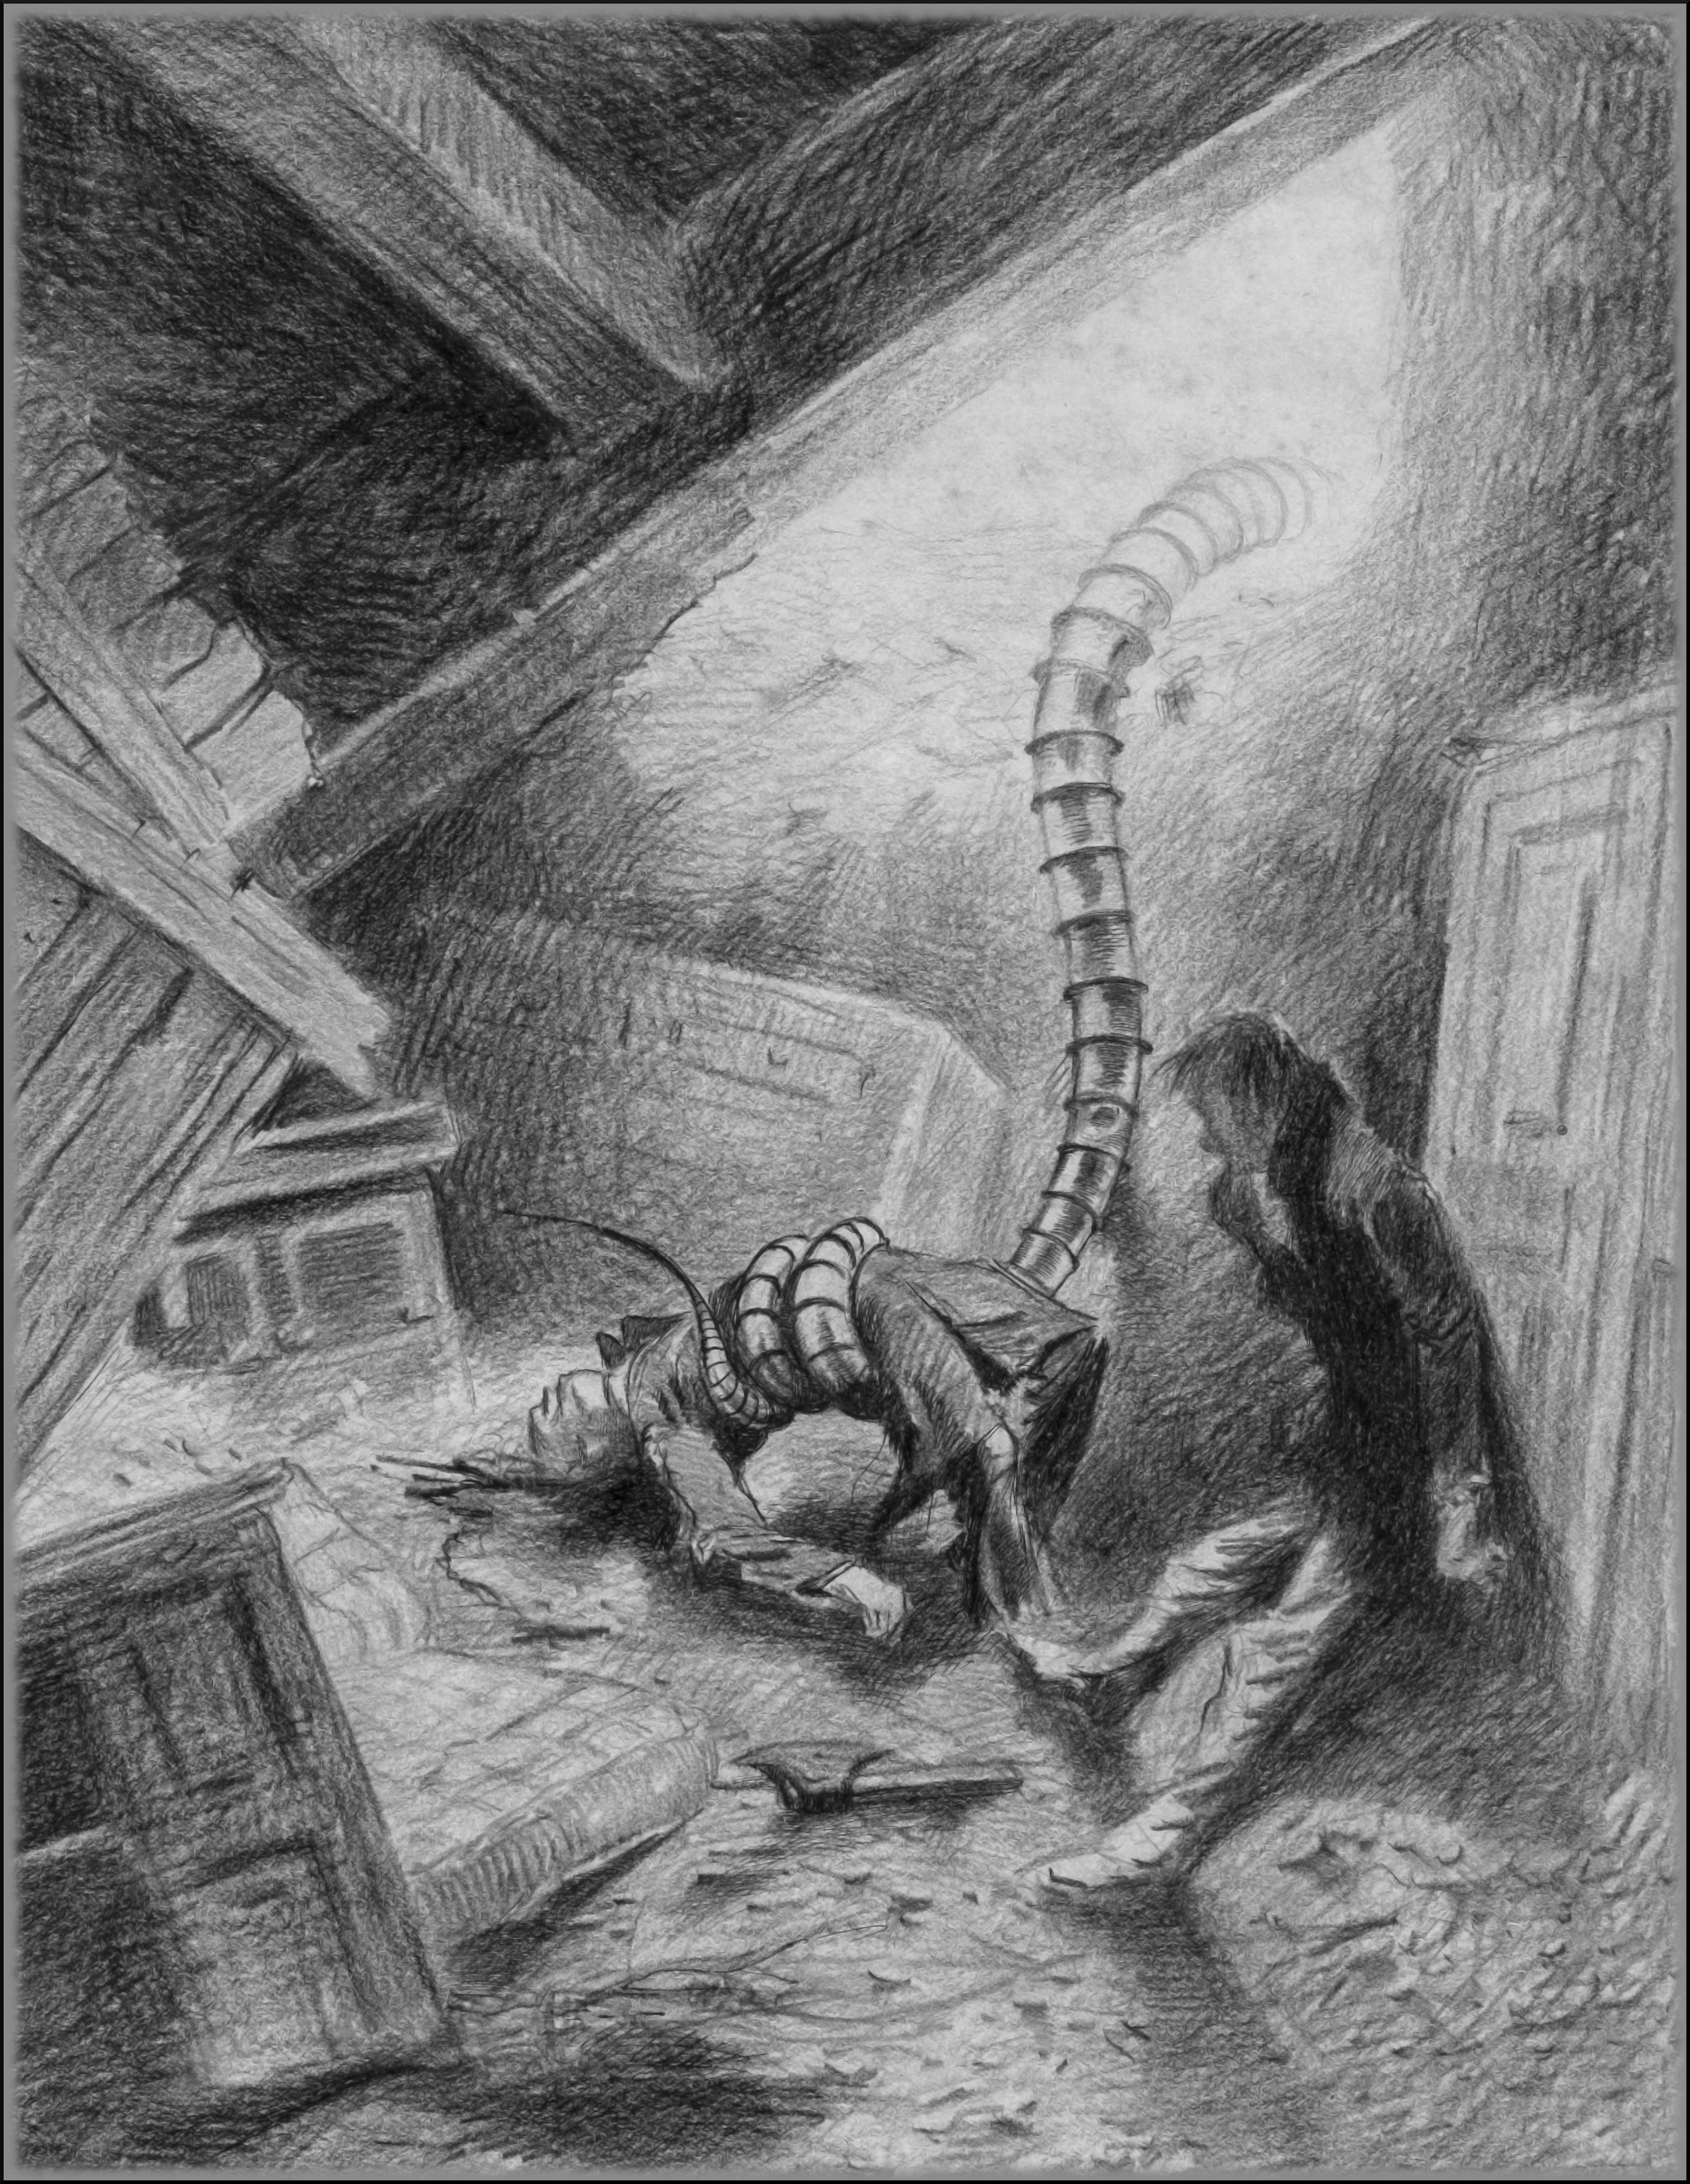
\includegraphics[width=\linewidth]{21dragged}
\caption{A heavy body was dragged across the floor}
\end{figure}

I crept back to the coal cellar, shut the door, and began to cover myself up as much as I could, and as noiselessly as possible in the darkness, among the firewood and coal therein. Every now and then I paused, rigid, to hear if the Martian had thrust its tentacles through the opening again.

Then the faint metallic jingle returned. I traced it slowly feeling over the kitchen. Presently I heard it nearer—in the scullery, as I judged. I thought that its length might be insufficient to reach me. I prayed copiously. It passed, scraping faintly across the cellar door. An age of almost intolerable suspense intervened; then I heard it fumbling at the latch! It had found the door! The Martians understood doors!

It worried at the catch for a minute, perhaps, and then the door opened.

In the darkness I could just see the thing—like an elephant's trunk more than anything else—waving towards me and touching and examining the wall, coals, wood and ceiling. It was like a black worm swaying its blind head to and fro.

Once, even, it touched the heel of my boot. I was on the verge of screaming; I bit my hand. For a time the tentacle was silent. I could have fancied it had been withdrawn. Presently, with an abrupt click, it gripped something—I thought it had me!—and seemed to go out of the cellar again. For a minute I was not sure. Apparently it had taken a lump of coal to examine.

I seized the opportunity of slightly shifting my position, which had become cramped, and then listened. I whispered passionate prayers for safety.

Then I heard the slow, deliberate sound creeping towards me again. Slowly, slowly it drew near, scratching against the walls and tapping the furniture.

While I was still doubtful, it rapped smartly against the cellar door and closed it. I heard it go into the pantry, and the biscuit-tins rattled and a bottle smashed, and then came a heavy bump against the cellar door. Then silence that passed into an infinity of suspense.

Had it gone?

At last I decided that it had.

It came into the scullery no more; but I lay all the tenth day in the close darkness, buried among coals and firewood, not daring even to crawl out for the drink for which I craved. It was the eleventh day before I ventured so far from my security.

%\begin{figure}[b!]
%\centering
%
\includegraphics[width=.5\textwidth]{25zombie}\captionlistentry{Tailpiece to Chapter \thechapter}
%\end{figure}